\section{Learning \& Training Dynamics}

\subsection*{\textcolor{primaryteal}{Q: What is the role of Batch Normalization (BN) in training neural networks?}}
\textbf{Batch Normalization} normalizes the input of each layer to have zero mean and unit variance across a mini-batch. This reduces internal co-variate shift (changes in the distribution of layer inputs during training), speeds up convergence, and stabilizes activation distributions and gradients.

\textbf{Mathematical Formulation}: For a mini-batch $B$ of size $m$:
\[
\mu_B = \frac{1}{m} \sum_{i=1}^{m} x_i, \quad \sigma_B^2 = \frac{1}{m} \sum_{i=1}^{m} (x_i - \mu_B)^2
\]
\[
\hat{x}_i = \frac{x_i - \mu_B}{\sqrt{\sigma_B^2 + \epsilon}}, \quad y_i = \gamma \hat{x}_i + \beta
\]
where $\epsilon$ is a small constant for numerical stability, and $\gamma, \beta$ are learnable parameters.

\subsection*{\textcolor{primaryteal}{Q: Why are learnable scale and shift parameters ($\gamma, \beta$) included in BN?}}
BN restricts the distribution of outputs into the same fixed distribution (mean=0, variance=1), which prevents the network from learning the optimal scale and bias. These parameters allow the network to undo the normalization if necessary, preserving representational power after the input is normalized.

\textbf{Parameter Learning}: The parameters $\gamma$ and $\beta$ are learned during training:
\[
\gamma = \text{Var}[x]^{1/2}, \quad \beta = \mathbb{E}[x]
\]
This allows the network to recover the original distribution if it's optimal for the task.

\subsection*{\textcolor{primaryteal}{Q: Where should BN be applied in a neural network?}}
\textbf{Batch Normalization} is typically applied after the affine transformation (like a linear or convolutional layer) and before the activation function such as ReLU. BN normalizes the pre-activation values which stabilizes the distribution before they pass through nonlinearities, which keeps gradients flowing smoothly during backpropagation. BN, typically, is not applied to the output layers.

\textbf{Reasoning}: BN should normalize the inputs to activation functions, as activations like ReLU are sensitive to input distribution shifts. Normalizing pre-activations ensures the activation function receives well-distributed inputs.

\subsection*{\textcolor{primaryteal}{Q: What are the limitations of BN with small batch sizes?}}
Small batch sizes lead to noisy estimates of the mean and variance, which can destabilize training and degrade performance. This may result in issues such as batch-wise overfitting or jittery parameter updates. Additionally, Batch Normalization loses much of its regularization effect when batch statistics become unreliable. In practice, a "small batch" typically refers to fewer than 32 samples per batch per device.

\textbf{Statistical Analysis}: The variance of the batch statistics scales as $\text{Var}[\mu_B] = \frac{\sigma^2}{m}$, so smaller batches lead to noisier estimates.

\subsection*{\textcolor{primaryteal}{Q: How does batch normalization work during inference?}}
During inference, batch normalization (BN) uses the running averages of the mean and variance computed during training, rather than calculating them from the current batch of data. This ensures deterministic outputs regardless of batch size. However, the outputs during inference may differ slightly from those during training due to the shift from batch-wise statistics to running estimates.

\textbf{Running Statistics Update}: The running statistics are updated during training as:
\[
\mu_{\text{running}} \leftarrow \alpha \mu_{\text{running}} + (1-\alpha) \mu_B
\]
\[
\sigma^2_{\text{running}} \leftarrow \alpha \sigma^2_{\text{running}} + (1-\alpha) \sigma^2_B
\]
where $\alpha$ is typically 0.9 or 0.99.

\subsection*{\textcolor{primaryteal}{Q: How do BatchNorm, LayerNorm, GroupNorm, and InstanceNorm compare?}}
\begin{figure}[H]
	\centering
	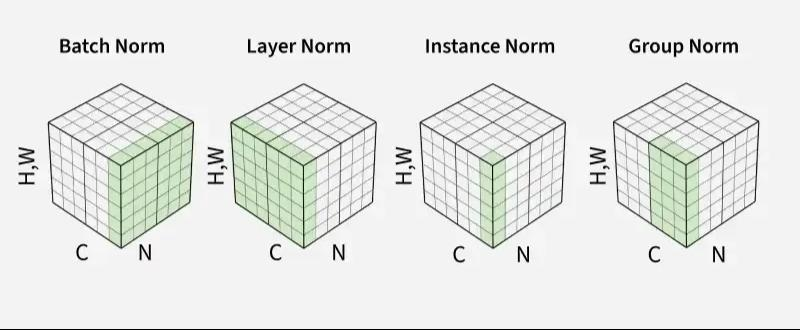
\includegraphics[width=0.8\textwidth]{norms.jpg}
	\caption{Source: \textit{https://www.geeksforgeeks.org/deep-learning/what-is-group-normalization/}}
\end{figure}

\begin{itemize}
	\item \textbf{Batch Normalization (BatchNorm)}: BatchNorm normalizes inputs across the batch dimension for each feature channel. It works well with large batch sizes and helps stabilize and accelerate training, but it can perform poorly with small batches and behaves differently during inference.
	
	\item \textbf{Layer Normalization (LayerNorm)}: LayerNorm normalizes across all feature dimensions within a single data sample. It is independent of batch size (robust for small batches) and is commonly used in architectures like Transformers and RNNs, but it tends to be less effective in convolutional neural networks.
	
	\item \textbf{Group Normalization (GroupNorm)}: GroupNorm divides channels into smaller groups and normalizes within each group. It performs consistently regardless of batch size and is particularly effective for convolutional models, though it requires tuning the number of groups (e.g., num groups=32).
	
	\item \textbf{Instance Normalization (InstanceNorm)}: InstanceNorm normalizes each individual sample and channel across spatial dimensions. It is widely used in style transfer applications as it helps remove instance-specific contrast information, but it may hurt performance in classification tasks where style information is important.
\end{itemize}

\textbf{Summary}: The choice of normalization method depends heavily on the task and batch size. For convolutional neural networks (CNNs) trained on large datasets like ImageNet, \textbf{BatchNorm} is the preferred choice. In scenarios with small batch sizes, such as object detection or segmentation, \textbf{GroupNorm} is typically more stable and effective. For natural language processing (NLP) and Transformer-based architectures, \textbf{LayerNorm} is widely used due to its batch-size independence. Finally, in style transfer or generative adversarial networks (GANs), \textbf{InstanceNorm} is favored for its ability to discard contrast and style-specific information.

\subsection*{\textcolor{primaryteal}{Q: What are the differences between SGD and Adam?}}
\textbf{SGD (Stochastic Gradient Descent)} uses a fixed or scheduled learning rate and is memory-efficient. The update rule is:
\[
\theta_{t+1} = \theta_t - \eta_t \nabla_\theta J(\theta_t)
\]
where $\eta_t$ is the learning rate at step $t$.

\textbf{Adam (Adaptive Moment Estimation)} adapts learning rates for each parameter and converges faster but may overfit. It maintains exponential moving averages of gradients and squared gradients:
\[
m_t = \beta_1 m_{t-1} + (1-\beta_1) \nabla_\theta J(\theta_t)
\]
\[
v_t = \beta_2 v_{t-1} + (1-\beta_2) (\nabla_\theta J(\theta_t))^2
\]
\[
\hat{m}_t = \frac{m_t}{1-\beta_1^t}, \quad \hat{v}_t = \frac{v_t}{1-\beta_2^t}
\]
\[
\theta_{t+1} = \theta_t - \frac{\eta}{\sqrt{\hat{v}_t} + \epsilon} \hat{m}_t
\]

\textbf{Key Insight}: Adam typically converges faster but may generalize less well than SGD with proper learning rate scheduling.

\subsection*{\textcolor{primaryteal}{Q: What is the role of momentum in SGD?}}
\textbf{Momentum} accumulates past gradients to smooth updates and accelerate convergence, especially in consistent gradient directions, and dampen oscillations caused by noisy gradients.

\textbf{Mathematical Formulation}: The momentum update rule is:
\[
v_{t+1} = \mu v_t - \eta \nabla_\theta J(\theta_t)
\]
\[
\theta_{t+1} = \theta_t + v_{t+1}
\]
where $\mu$ is the momentum coefficient (typically 0.9).

\textbf{Benefits of Momentum}:
\begin{itemize}
	\item Accelerating convergence in consistent gradient directions
	\item Reducing oscillations in narrow valleys
	\item Improving training stability
	\item Helping escape local minima
\end{itemize}

\subsection*{\textcolor{primaryteal}{Q: What are advanced optimization techniques beyond Adam?}}
Several advanced optimizers have been developed to address limitations of Adam:

\begin{itemize}
	\item \textbf{AdamW}: Decouples weight decay from gradient-based updates, leading to better generalization
	\item \textbf{RAdam}: Rectifies the variance of adaptive learning rates, providing more stable training
	\item \textbf{Lion}: Uses sign-based updates with momentum, achieving competitive performance with fewer parameters
	\item \textbf{AdaBelief}: Adapts step sizes based on belief in observed gradients, improving convergence
\end{itemize}

\subsection*{\textcolor{primaryteal}{Q: How can overfitting be reduced in machine learning?}}
Overfitting occurs when a model learns the training data too well, including noise, leading to poor generalization. Several techniques can help:

\begin{itemize}
	\item \textbf{Regularization}: Adding penalty terms to the loss function
	\item \textbf{Early Stopping}: Monitoring validation performance and stopping when it degrades
	\item \textbf{Data Augmentation}: Creating additional training examples through transformations
	\item \textbf{Dropout}: Randomly deactivating neurons during training
	\item \textbf{Cross-validation}: Using multiple train/validation splits
\end{itemize}

\subsection*{\textcolor{primaryteal}{Q: What is the difference between L1 and L2 regularization?}}
Both L1 and L2 regularization add penalty terms to prevent overfitting, but they have different effects:

\textbf{L1 Regularization (Lasso)}: Adds $\lambda \sum_{i=1}^{n} |w_i|$ to the loss function
\begin{itemize}
	\item Promotes sparsity by driving some weights to exactly zero
	\item Useful for feature selection
	\item Less robust to outliers
\end{itemize}

\textbf{L2 Regularization (Ridge)}: Adds $\lambda \sum_{i=1}^{n} w_i^2$ to the loss function
\begin{itemize}
	\item Prevents any weight from becoming too large
	\item More robust to outliers
	\item All features contribute to the model
\end{itemize}

\subsection*{\textcolor{primaryteal}{Q: How does dropout work?}}
\textbf{Dropout} is a regularization technique that randomly sets a fraction of neurons to zero during training:

\begin{itemize}
	\item During training: Each neuron is dropped with probability $p$ (typically 0.5)
	\item During inference: All neurons are active, but weights are scaled by $(1-p)$
	\item Effect: Prevents co-adaptation of neurons and improves generalization
\end{itemize}

\subsection*{\textcolor{primaryteal}{Q: Why does dropout improve generalization?}}
Dropout improves generalization through several mechanisms:

\begin{itemize}
	\item \textbf{Prevents Co-adaptation}: Neurons cannot rely on specific combinations of other neurons
	\item \textbf{Ensemble Effect}: Each forward pass uses a different subnetwork, creating an implicit ensemble
	\item \textbf{Regularization}: Forces the network to be robust to missing information
	\item \textbf{Reduces Overfitting}: Limits the network's capacity to memorize training data
\end{itemize}

\subsection*{\textcolor{primaryteal}{Q: What are common activation functions and when to use them?}}
\begin{figure}[H]
	\centering
	\includegraphics[width=0.8\textwidth]{activation.png}
	\caption{Common activation functions and their properties}
\end{figure}

\begin{itemize}
	\item \textbf{Sigmoid}: Outputs values between 0 and 1, useful for binary classification
	\item \textbf{Tanh}: Outputs values between -1 and 1, zero-centered, better for hidden layers
	\item \textbf{ReLU}: Most popular, computationally efficient, helps with vanishing gradients
	\item \textbf{Leaky ReLU}: Addresses dying ReLU problem by allowing small negative gradients
	\item \textbf{Softmax}: Outputs probability distribution, used in multi-class classification
	\item \textbf{GELU}: Smooth approximation of ReLU, used in modern architectures
	\item \textbf{Swish}: Self-gated activation, often outperforms ReLU
\end{itemize}

\subsection*{\textcolor{primaryteal}{Q: When should you use Sigmoid vs Softmax?}}
The choice between Sigmoid and Softmax depends on the task:

\textbf{Sigmoid}: Use for binary classification or when you need independent probabilities
\begin{itemize}
	\item Outputs values between 0 and 1
	\item Each output is independent of others
	\item Suitable for multi-label classification
\end{itemize}

\textbf{Softmax}: Use for multi-class classification when outputs should sum to 1
\begin{itemize}
	\item Outputs probability distribution that sums to 1
	\item Outputs are dependent (compete with each other)
	\item Suitable for single-label classification
\end{itemize}

\subsection*{\textcolor{primaryteal}{Q: What is gradient flow and why is it important?}}
\textbf{Gradient flow} refers to how gradients propagate backward through the network during training:

\begin{itemize}
	\item \textbf{Vanishing Gradients}: Gradients become very small in deep networks, slowing learning
	\item \textbf{Exploding Gradients}: Gradients become very large, causing unstable training
	\item \textbf{Importance}: Proper gradient flow is essential for training deep networks effectively
\end{itemize}

\textbf{Solutions}:
\begin{itemize}
	\item Proper weight initialization
	\item Batch normalization
	\item Residual connections
	\item Careful choice of activation functions
\end{itemize}

\subsection*{\textcolor{primaryteal}{Q: What are advanced weight initialization strategies?}}
Proper weight initialization is crucial for training deep networks:

\begin{itemize}
	\item \textbf{Xavier/Glorot}: Scales weights by $\sqrt{\frac{2}{n_{in} + n_{out}}}$ for sigmoid/tanh
	\item \textbf{He}: Scales weights by $\sqrt{\frac{2}{n_{in}}}$ for ReLU activations
	\item \textbf{Orthogonal}: Initializes weights as orthogonal matrices, preserving gradient norms
	\item \textbf{LSUV}: Layer-sequential unit-variance initialization for better training dynamics
\end{itemize}

\subsection*{\textcolor{primaryteal}{Q: What are curriculum learning and learning rate scheduling?}}
\textbf{Curriculum learning} presents training examples in a meaningful order, starting with simpler examples and gradually increasing difficulty.

\textbf{Mathematical Formulation}: For a curriculum function \(c(t)\) that determines difficulty at step \(t\):
\[
\text{Difficulty}(t) = c(t) \cdot \text{MaxDifficulty}
\]

\textbf{Learning Rate Scheduling} adjusts the learning rate during training:
\begin{itemize}
	\item \textbf{Step Decay}: Reduces learning rate by a factor every N epochs
	\item \textbf{Exponential Decay}: Continuously decreases learning rate exponentially
	\item \textbf{Cosine Annealing}: Smoothly decreases learning rate following cosine curve
	\item \textbf{One Cycle}: Increases then decreases learning rate in a single cycle
\end{itemize}

\subsection*{\textcolor{primaryteal}{Q: What are advanced regularization techniques?}}
Beyond L1/L2 and dropout, several advanced regularization techniques exist:

\begin{itemize}
	\item \textbf{Label Smoothing}: Replaces hard labels with soft probability distributions
	\item \textbf{Mixup}: Creates new training examples by interpolating between pairs
	\item \textbf{CutMix}: Combines parts of different images for data augmentation
	\item \textbf{Stochastic Depth}: Randomly drops entire layers during training
	\item \textbf{ShakeDrop}: Applies random scaling to residual connections
\end{itemize}

\textbf{Mathematical Benefits}:
\begin{itemize}
	\item Improved generalization through better calibration
	\item Enhanced robustness to adversarial examples
	\item Better handling of label noise
	\item Reduced overfitting in deep networks
\end{itemize}
